\documentclass[12pt]{article}

\usepackage{hyperref}
\usepackage{fontspec}
\usepackage{polyglossia}
\usepackage{xcolor} 
\usepackage{graphicx}
\usepackage[final]{pdfpages}

\setdefaultlanguage{malayalam}
\setmainfont[Script=Malayalam,HyphenChar="00AD]{Gayathri}
\sloppy
\usepackage{color}
\usepackage{xcolor}
\definecolor{dark-red}{rgb}{0.4,0.15,0.15}
\definecolor{dark-blue}{rgb}{0.15,0.15,0.8}
\definecolor{medium-blue}{rgb}{0,0,0.5}
\hypersetup{
	colorlinks, linkcolor={dark-blue},
	citecolor={dark-blue}, urlcolor={medium-blue}
}


\begin{document}
	
\begin{titlepage}
	\begin{center}
		\Large{{\textbf{ഗായത്രി ഫോണ്ട്}}}\\[2cm]

		
\includegraphics[scale=0.5]{logo.png}\\[0.5cm]	
		
		\textsc{\Large {സ്വതന്ത്രമലയാളം കമ്പ്യൂട്ടിങ്ങ്}}~\\[4cm]
		{\textsc{\Large {പ്രോജക്ട് റിപ്പോര്‍ട്ട്}}}\\
		നവംബര്‍ 2018
	\end{center}
\end{titlepage}
 

	
	
	%\tableofcontents
	
	\section{ഗായത്രി ഫോണ്ട് പ്രോജക്ട്}
	
	\subsection{ആമുഖം}
	
	\paragraph{}
	കേരള ഭാഷാ ഇന്‍സ്റ്റിറ്റ്യൂട്ടിന്റെ സാമ്പത്തിക സഹായത്തോടെ സ്വതന്ത്രമലയാളം കമ്പ്യൂട്ടിങ്ങ് നിര്‍മ്മിക്കുന്ന മലയാളം യൂണിക്കോഡ് ഫോണ്ടാണ് \textbf{ഗായത്രി}. ഫോണ്ടിന്റെ രൂപകല്പന ബിനോയ് ഡൊമിനിക്കിന്റേതാണ്. ഓപ്പണ്‍ടൈപ്പ് സാങ്കേതികവിദ്യ കാവ്യ മനോഹറും പ്രോജക്ട് മേല്‍നോട്ടം സന്തോഷ് തോട്ടിങ്ങലും നിര്‍വ്വഹിച്ചിരിക്കുന്നു.
	
	\paragraph{}
	റെഗുലര്‍, ബോള്‍ഡ്, തിന്‍ എന്നിങ്ങനെ മൂന്നു കനങ്ങളില്‍ ലഭ്യമായിരിക്കുന്ന ഗായത്രി, തലക്കെട്ടുകള്‍ക്ക് അനുയോജ്യമായ വിധം രൂപകല്പന ചെയ്തിരിക്കുന്ന ഫോണ്ടാണ്. എങ്കിലും ചെറിയ വലിപ്പത്തിലും സാമാന്യം നല്ല വായനാക്ഷമത ഗായത്രി ഫോണ്ടിനുണ്ട്. ഈ റിപ്പോര്‍ട്ട് പൂര്‍ണ്ണമായും ഗായത്രി ഫോണ്ടിലാണ് തയ്യാറാക്കിയിരിക്കുന്നത്.
	
	\subsection{ലിപി സഞ്ചയം}
	
	\paragraph{}
	
	യൂണിക്കോഡിന്റെ ഏറ്റവും പുതിയ പതിനൊന്നാം പതിപ്പിനെ ആധാരമാക്കിയാണ് ഗായത്രി നിര്‍മ്മിച്ചിട്ടുള്ളത്. മലയാളത്തില്‍ ഇന്ന് നിത്യോപയോഗത്തിലുള്ള സ്വരങ്ങളും വ്യഞ്ജനങ്ങളും ചില്ലക്ഷരങ്ങളും അക്കങ്ങളും കൂടാതെ പുരാതനമലയാളത്തില്‍ നിലനിന്നിരുന്ന അക്ഷരങ്ങളും അക്കങ്ങളുമെല്ലാം ചേര്‍ന്ന സമഗ്രമായ അക്ഷരക്കൂട്ടം ഗായത്രിയിലുണ്ട്. മലയാളത്തിലെ പുരാരേഖകള്‍ ഡിജിറ്റൈസ് ചെയ്യുമ്പോള്‍ അത്യന്താപേക്ഷിതമാണിവ. കാല്‍, അര, മുക്കാല്‍, പതിനാറില്‍ മൂന്ന് തുടങ്ങിയ ഭിന്നസംഖ്യാരൂപങ്ങളെ കുറിക്കുന്ന ൳, ൴, ൵, ൸  ഇവ ചില ഉദാഹരണങ്ങള്‍. മലയാളം യൂണിക്കോഡ് കവറേജ് ചിത്രം \ref{unicode} ല്‍ കാണാം.
	
	\begin{figure}
		\begin{centering}
			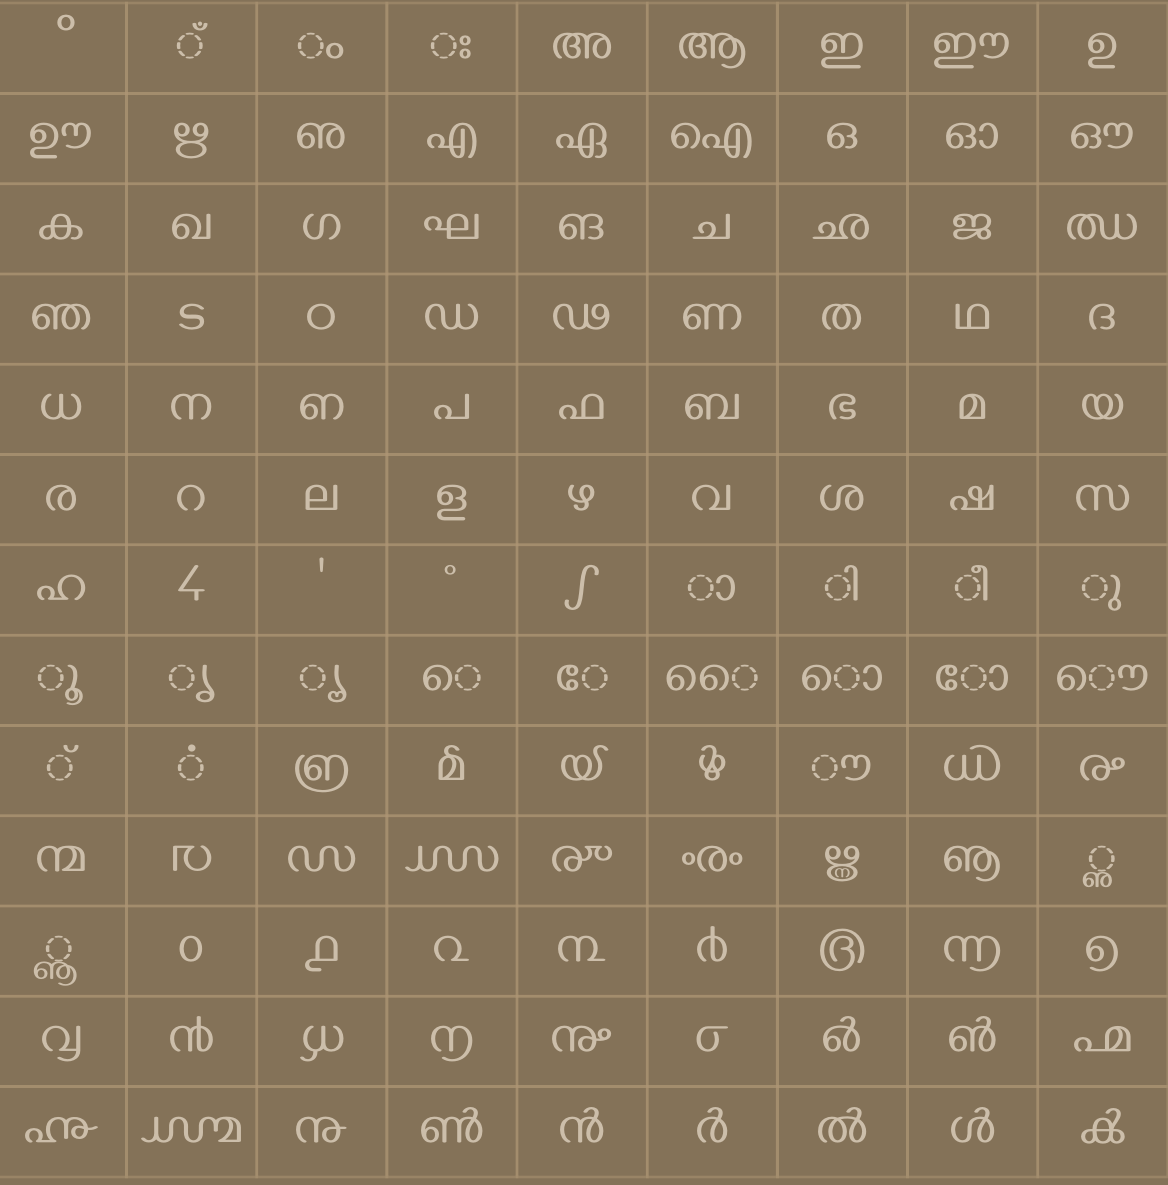
\includegraphics[width=0.8\textwidth]{ml-unicode.png}
			\caption{മലയാളം യൂണിക്കോഡ് സമ്പൂര്‍ണ്ണ കവറേജ്}
			\label{unicode}
		\end{centering}
	\end{figure}
	
	\paragraph{}
	മലയാളലിപിയിലെ കൂട്ടക്ഷരങ്ങളെ പരമാവധി ഉള്‍ക്കൊള്ളിച്ചുകൊണ്ടാണ് ഗായത്രിഫോണ്ടിന്റെ ഡിസൈന്‍. അതുകൊണ്ട് തന്നെ ഒരു സമഗ്രലിപിസഞ്ചയഫോണ്ടാണ് ഗായത്രി.
	
	\paragraph{}
	ഇന്ന് മലയാളരേഖകളില്‍ മലയാളത്തോടൊപ്പം ഇംഗ്ലീഷ് വാക്കുകളും കലര്‍ത്തിയെഴുതുന്നത് സര്‍വ്വ സാധാരണമാണ്. അതുകൊണ്ട് തന്നെ ആധുനികമലയാളം ഫോണ്ടുകളില്‍ മലയാളം ലിപിയുടെ ഡിസൈന് അനുരൂപമായ ഇംഗ്ലീഷുള്‍പ്പെടുന്ന ലാറ്റിന്‍ ലിപിയും അത്യാവശ്യമാണ്. ഗായത്രി ഫോണ്ടില്‍ ലാറ്റിന്‍ അക്ഷരങ്ങളും കൂടി അതുകൊണ്ടു തന്നെ ഉള്‍പ്പെടുത്തിയിട്ടുണ്ട്.  എല്ലാം ചേര്‍ന്ന് ആകെ 1116 ഗ്ലിഫുകള്‍ ഗായത്രിഫോണ്ടിലുണ്ട്. 
	
	\paragraph{}
	മലയാളത്തിലെ ചില അക്ഷരങ്ങള്‍ക്ക് സാര്‍വ്വത്രികമായി ഒരേ രൂപമല്ല ഉള്ളത്. 'ച്ച', 'കൂ', 'ള്ള' തുടങ്ങിയവയുടെ ശൈലീഭേദങ്ങളുള്‍ക്കൊണ്ടുകൊണ്ട് അവ കൂടി ഗായത്രി ഫോണ്ടില്‍ ചേര്‍ത്തിട്ടുണ്ട്. സോഫ്റ്റ്‌വെയര്‍ സഹായത്തോടെ ഇതിലേതുവേണമെന്നു തെരഞ്ഞെടുക്കാന്‍ ഉപയോക്താവിനാകും. ചിത്രം \ref{style} നോക്കുക. 
	‍ 
	\begin{figure}
		\begin{centering}
			
\includegraphics[width=0.8\textwidth]{style.jpg}
			\caption{ശൈലീഭേദങ്ങള്‍}
			\label{style}
		\end{centering}
	\end{figure}
	
	
	\subsection{ഡിസൈന്‍ സവിശേഷതകള്‍}
	
	ആമുഖത്തില്‍ സൂചിപ്പിച്ചിരിക്കുന്നതുപോലെ തലക്കെട്ടുകള്‍ക്ക് അനുയോജ്യമായ വിധമാണ് ഗായത്രിയുടെ ഡിസൈന്‍. അക്ഷരനാടയുടെ വീതിവിന്യാസം തുല്യമല്ല. സെരിഫ് ശൈലിയോടടുത്തുനില്‍ക്കുന്നതാണിത്. അക്ഷരങ്ങളുടെ അറ്റങ്ങള്‍ ഏതാണ്ട് ഉരുണ്ടിട്ടാണ്. വലിയ രൂപത്തില്‍ ഇവ വ്യക്തമായി കാണാവുന്ന മിഴിവാര്‍ന്ന ഡിസൈന്‍ സാദ്ധ്യതകള്‍ ഗായത്രിയ്ക്ക് നല്‍കാനാകും.  ചിത്രം \ref{one} നോക്കുക.
	
	\begin{figure}
		\begin{centering}
			
\includegraphics[width=0.8\textwidth]{ga.jpg}
			\caption{ഡിസൈന്‍ വിശദാംശങ്ങള്‍}
			\label{one}
		\end{centering}
	\end{figure}
	
	\paragraph{}
	പുസ്തകങ്ങളുടേയും ആനുകാലികങ്ങളുടേയുമെല്ലാം ലേയൗട്ട് തയ്യാറാക്കുമ്പോള്‍ പല കനത്തിലുള്ള ഫോണ്ട് വേരിയന്റുകള്‍ ആവശ്യമായി വരാറുണ്ട്. ഇതിനായി മൂന്നുകനങ്ങളില്‍ - ബോള്‍ഡ്, റെഗുലര്‍, തിന്‍- ഗായത്രി അക്ഷരരൂപങ്ങള്‍ ലഭ്യമാണ്. ചിത്രം \ref{variants} നോക്കുക.
	
	\begin{figure}
		\begin{centering}
			
\includegraphics[width=0.7\textwidth]{variant.jpg}
			\caption{ബോള്‍ഡ്, റെഗുലര്‍, തിന്‍: മൂന്നു വേരിയന്റുകള്‍}
			\label{variants}
		\end{centering}
	\end{figure}
	
	\subsection{നിര്‍മ്മാണവും ലൈസന്‍സിങ്ങും}
	
	\paragraph{}
	ഗായത്രി ഫോണ്ട് നിര്‍മ്മാണം പൂര്‍ണ്ണമായും ഓപ്പണ്‍സോഴ്സ് സോഫ്റ്റ്‌വെയര്‍ ഡെവലപ്മെന്റ് മാതൃകയിലാണ് പൂര്‍ത്തിയായിരിക്കുന്നത്. ഡിസൈനര്‍ അക്ഷരങ്ങളുടെ ബോള്‍ഡ്, റെഗുലര്‍, തിന്‍ ശൈലികളിലുള്ള വെക്ടര്‍ ഇമേജുകള്‍ തയ്യാറാക്കുന്നു. ഇവയെ UFO(Unified Font Object) ഫോര്‍മാറ്റിലുള്ള ഗ്ലിഫ് ഫയലുകള്‍ ആക്കുകയാണ് ഫോണ്ട് എഞ്ചിനീയറിങ്ങിലെ ആദ്യ പടി. പിന്നീട് കൂട്ടക്ഷരങ്ങള്‍ കൃത്യമായി ചിത്രീകരിക്കാനാവശ്യമായ ഓപ്പണ്‍ടൈപ്പ് എഞ്ചിനീയറിങ്ങ് നിയമങ്ങള്‍ ചേര്‍ത്ത് ബില്‍ഡ് ചെയ്ത് OTF, TTF, WOFF ഫോര്‍മറ്റിലുള്ള ഫോണ്ടുകള്‍ നിര്‍മ്മിക്കുന്നു. ഈ ഫോര്‍മാറ്റുകളിലെല്ലാമുള്ള ബോള്‍ഡ്, റെഗുലര്‍, തിന്‍ ഫോണ്ടുകള്‍ സ്വതന്ത്രമലയാളംകമ്പ്യൂട്ടിങ്ങിന്റേയും (\url{https://smc.org.in/fonts/}) കേരളഭാഷാഇന്‍സ്റ്റിറ്റ്യൂട്ടിന്റേയും വെബ്സൈറ്റൂകളില്‍ നിന്നും ഡൗണ്‍ലോഡ് ചെയ്യാന്‍ ലഭ്യമാകും.
	
	\paragraph{}
	ഫോണ്ടിന്റെ സോഴ്സ് കോഡ് ഓപ്പണാണ്. അതായത്, വരച്ച അക്ഷരരൂപങ്ങളുടെ വെക്ടര്‍ ഇമേജുകള്‍ (svg format), ഇവയില്‍ നിന്നും തയ്യാറാക്കിയ ഗ്ലിഫ് ഫയലുകള്‍, ഓപ്പണ്‍ടൈപ്പ് എഞ്ചിനീയറിങ്ങ് നിയമങ്ങള്‍ ഇവയെല്ലാം നിര്‍മ്മാണഘട്ടത്തില്‍ ഇതുവരെ വരുത്തിയ മാറ്റങ്ങളുള്‍പ്പെടെ ഇവിടെ (\url{https://gitlab.com/smc/fonts/gayathri/}) ലഭ്യമാണ്.
	
	\paragraph{}
		ഓപ്പണ്‍ ഫോണ്ട് ലൈസന്‍സിലാണ് ഗായത്രി ഫോണ്ട് പുറത്തിറക്കിയിരിക്കുന്നത്. സ്വതന്ത്രമലയാളം കമ്പ്യൂട്ടിങ്ങും കേരളഭാഷാഇന്‍സ്റ്റിറ്റ്യൂട്ടും ചേര്‍ന്ന് ഫോണ്ടിന്റെ പകര്‍പ്പവകാശം പങ്കുവെയ്ക്കുന്നു.
	
	\section{ഗായത്രി ഡിജിറ്റല്‍ ഫോണ്ട്: സാങ്കേതിക വിശദാംശങ്ങള്‍}
	
	\subsection{ഫോണ്ടിലെ യൂണിക്കോഡ് പോയിന്റുകള്‍}
	ഗായത്രി ഫോണ്ടില്‍ ഉള്‍ക്കൊള്ളിച്ചിട്ടുള്ള മുഴുവന്‍ യൂണിക്കോഡ് പോയിന്റുകളുടെയും പട്ടിക ഇനിയുള്ള താളുകളില്‍ നല്‍കിയിരിന്നുന്നു.
	
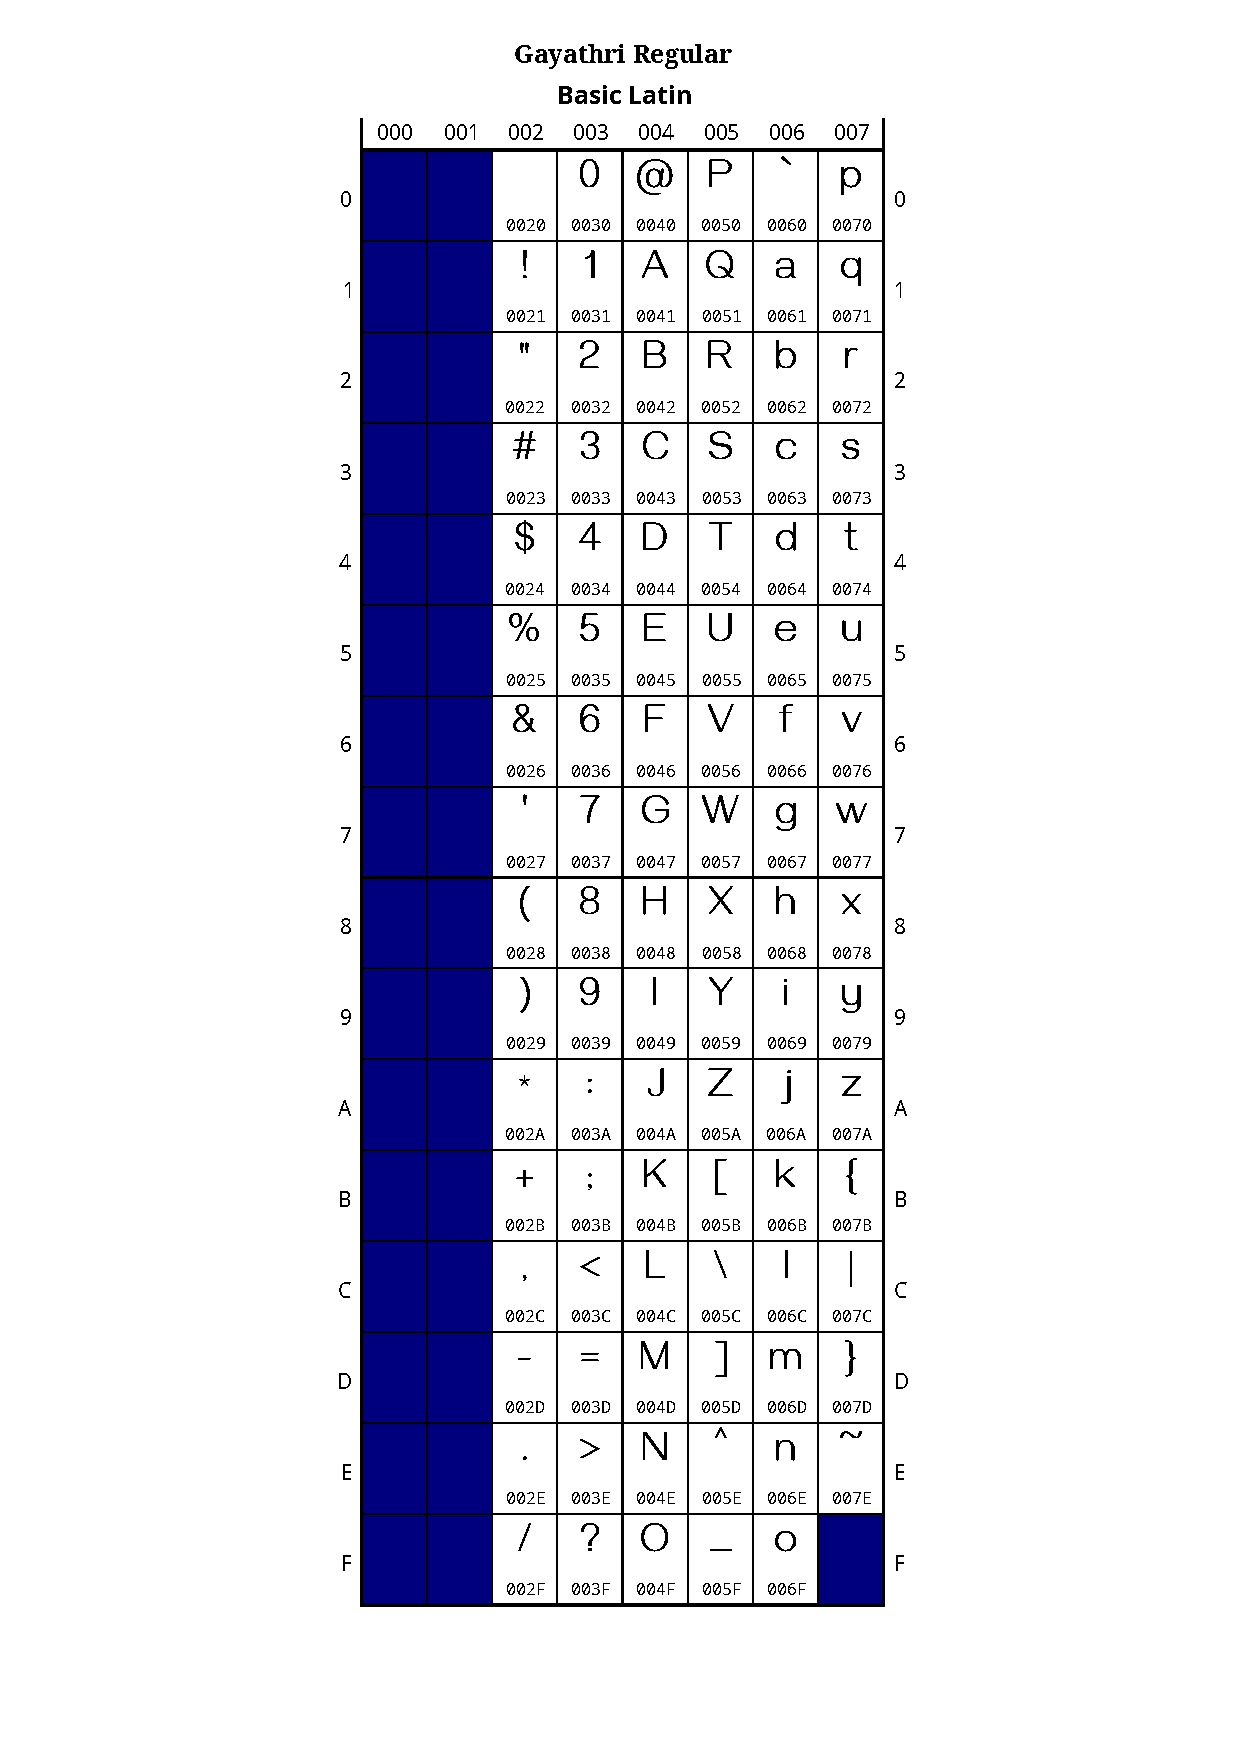
\includepdf[pages=-]{Gayathri-Regular-table.pdf}

	\subsection{ഫോണ്ടിലെ ഗ്ലിഫുകളുടെ പട്ടിക}
		ഇവിടെ ചേര്‍ക്കണം
	
	\section{ഗായത്രി ഫോണ്ട്: ഉപയോഗ സാദ്ധ്യതകള്‍}
	
	ഫോണ്ട് ഉപയോഗിക്കാവുന്ന ചില രീതികള്‍ ഇവിടെ ചേര്‍ക്കണം. നല്ല മാതൃകകള്‍ ചേര്‍ക്കണം.
	
\includepdf[pages=-]{usecase.pdf}
	
	
\end{document}


 
